\documentclass{beamer} 
% \usetheme{Goettingen} 

\usepackage[latin1]{inputenc} 
\usepackage[ngerman]{babel} 
\usepackage[orientation=landscape,size=custom,width=16,height=9,scale=0.5]{beamerposter}
\usepackage{beamerthemeshadow}
\setbeamertemplate{enumerate items}[ball]

\begin{document}
\title{Producer/Consumer-Pattern}  
\author{Matthias Seifert}
\date{\today} 

\begin{frame}
\titlepage
\end{frame}
%tableofcontent
\section{Aufgabe}
\begin{frame}
\begin{block}{die Aufgabe}
Mehrere Threads sollen miteinander kommunizieren k�nnen und f�r den
Austausch von Nachrichten einen Puffer verwenden.
\end{block}
\end{frame}
\begin{frame}
\centering
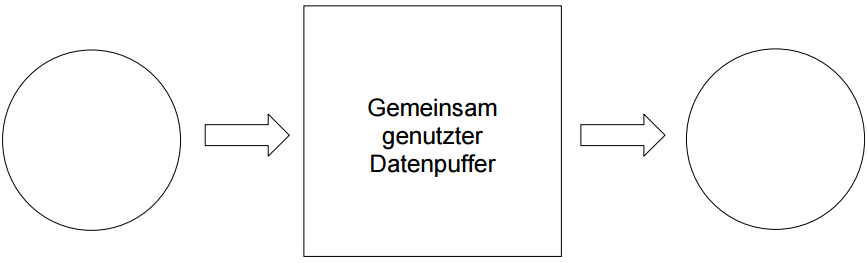
\includegraphics[width=.9 \textwidth]{img/1-1ohne.png}
\end{frame}

\begin{frame}
\centering
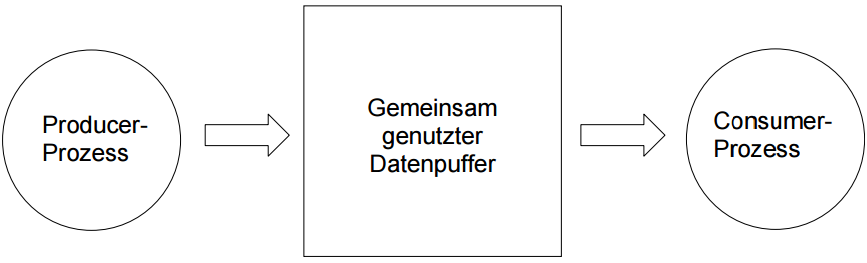
\includegraphics[width=.9 \textwidth]{img/1-1mit.png}
\end{frame}

\begin{frame}
\centering
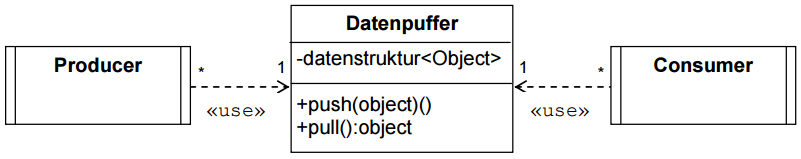
\includegraphics[width=.9 \textwidth]{img/klassendiagramm.png}
\end{frame}


\begin{frame}
\begin{block}{Problem}
Producer und Consumer d�rfen nicht gleichzeitig auf ein Element zugreifen
\end{block}
\end{frame}

\section{die L�sung}
\begin{frame}
\begin{block}{kritische Abschnitte sch�tzen}
\setbeamertemplate{itemize items}[square]
\begin{itemize}
  \item Semaphore
  \pause
  \item hier: Monitor
\pause
   \begin{itemize}
     \item<1-> zu sch�tzendes Element wird im Monitor verborgen
     \item<2-> Threads die einen blockierten Abschnitt betreten wollen werden
     blockiert.
 \end{itemize}
\end{itemize}
\end{block}
\end{frame}

\begin{frame}
\centering
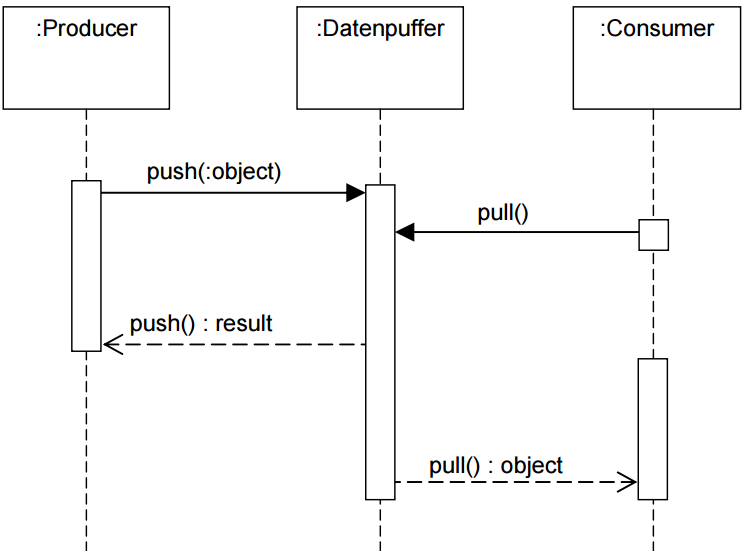
\includegraphics[height=.9 \textheight]{img/sequenz.png}
\end{frame}

\begin{frame}

\begin{columns}
\begin{column}{.5\textwidth}
\begin{block}{Vorteile}
\setbeamertemplate{itemize items}[square]
\begin{itemize}
  \item Producer und Consumer sind entkoppelt
  \item Anzahl Producer und Consumer kann unterschiedlich sein
  \item Konsistenz der Daten ist Gew�hrleistet
\end{itemize}
\end{block}
\end{column}
\begin{column}{.5\textwidth}
\begin{block}{Nachteile}
\setbeamertemplate{itemize items}[square]
\begin{itemize}
  \item Unbekannte Ausf�hrungsreihenfolge bei Freigabe von Element
\end{itemize}
\end{block}
\end{column}
\end{columns}
\end{frame}
\section{�hnliche Muster}
\subsection{Pipes \& Filters}
\begin{frame}

\begin{columns}
\begin{column}{.5\textwidth}
\begin{block}{Pipes \& Filters}
\setbeamertemplate{itemize items}[square]
\begin{itemize}
\item Sonderfall mit einem Producer und einem Consumer
\item Pipes = Pufferspeicher
\end{itemize}
\end{block}
\end{column}
\begin{column}{.5\textwidth}
\centering
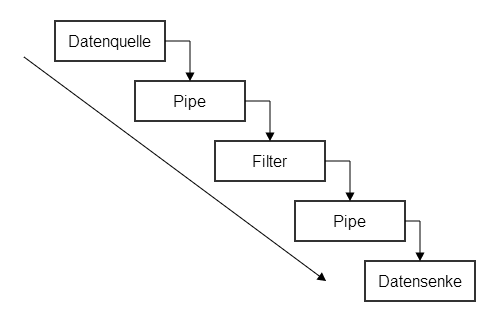
\includegraphics[width=.8\textwidth]{img/PipesAndFilters.png}
\end{column}
\end{columns}
\end{frame}

\subsection{Guarded Suspension}
\begin{frame}

\begin{block}{Guarded Suspension}
\setbeamertemplate{itemize items}[square]
\begin{itemize}
\item Objekt muss zum Objektaufruf in definiertem Zustand sein
\item zugreifende Objekte m�ssen warten bis das Objekt in diesem Zustand ist
\end{itemize}
\end{block}

\end{frame}



% \subsection{Guarded Suspension}
% \begin{frame}
% asd
% \end{frame}



\end{document}